\documentclass[12pt]{article}

\usepackage{graphicx}
\usepackage[hidelinks, colorlinks = true, urlcolor = blue, citecolor = black]{hyperref}

%opening
\title{Homework 2 - Venice Boat Classification\\
	\large Machine Learning 2018-19 - Sapienza}
\author{Luigi Russo 1699981}

\begin{document}
	
\maketitle
\newpage
\tableofcontents
\newpage
\section{Introduction}
This is my report for the second homework of Machine Learning course, about the Venice Boat Classification. First of all I will point out which have been the goals of this homework, starting of course from defining the specific classification problem (view section \ref{sec:image_classification_problem}) that I have chosen to focus on. After defining the kinds of algorithms that I have implemented and used (view section \ref{sec:models}), I will describe the dataset (view section \ref{sec:dataset}) and how I have handled the preprocessing phase (view section \ref{sec:preprocessing}). I will finally present the results of the evaluation phase (view section \ref{sec:results}).

\subsection{Learning goals}
\subsubsection{Classification problem}
\label{sec:image_classification_problem}
I have decided to focus on the problem of classifying \textbf{18} different classes of Venice boats. Given an instance of image, I want to be able to compute which is the correct type of boat of the input image. I have decided to use a pretrained model (Inception v3) in order to extract the features of each image: at this point, the feature vector is passed to some classifiers, such as SVM classifier. The model can be finally tested, computing the accuracy and it is possible to plot the confusion matrix.
\subsubsection{Metrics}
The main goal of this homework is to correctly classify the highest number of input images, for this reason I will take into account both accuracy and precision metrics.
\subsubsection{Many models}
\label{sec:models}
As in the first homework, also in this one I will give great importance to the comparison between different models. Once the pretrained graph extracts the features vector of the input image, it is passed to some classifier that actually runs the last step of the classification. I have decided to compare these 6 different classifiers:
\begin{itemize}
	\item Support Vector Machine (\textbf{SVM})
	\item Extra Trees (\textbf{ET})
	\item Random Forest (\textbf{RF})
	\item K-Nearest Neighbor (\textbf{KNN})
	\item Multi-Layer Perceptron (\textbf{ML})
	\item Gaussian Binomial (\textbf{GNB})
\end{itemize}

\section{Tools used}
I have used Python 3.6 programming language, because of its well-documented modules and libraries: I did not want to reinvent the wheel, so I have used the well-known \textit{Scikit-Learn}, \textit{Numpy}, \textit{Matplotlib} libraries to build, train, and evaluate the classifier. In the next sections I will give further details on the precise methods used.
I have provided the source-code as a collection of Python files (extension .py). It is possible to view the source-code in the attached zipped file (it is also present \href{https://www.gitlab.com/lrusso96/machine-learning}{in this GitLab repository}).

\section{The pretrained model}
Since I have decided to use a pretrained model to extract features, I have downloaded and reused a checkpoint of the Inception v3 model \cite{Inception}. Inception-v3 is trained for the ImageNet Large Visual Recognition Challenge using the data from 2012, and has a 78.0\% top-1 accuracy and a 93.9\% top-5 accuracy over the 1000 classes of Imagenet. In particular I have used the checkpoint of 12/05/2015, saving it in the 'pretrained' folder. This file (extension .pb) cannot be directly used, but it has to be imported, when initializing the TensorFlow session: this is possible thanks to some TensorFlow functions: \textit{ParseFromString} and \textit{import\_graph\_def}; the first one simply transforms a binary file into a complex graph object, instead the second one actually makes the graph available to the current TensorFlow session.

\begin{figure}[!ht]
	\centering % optional
	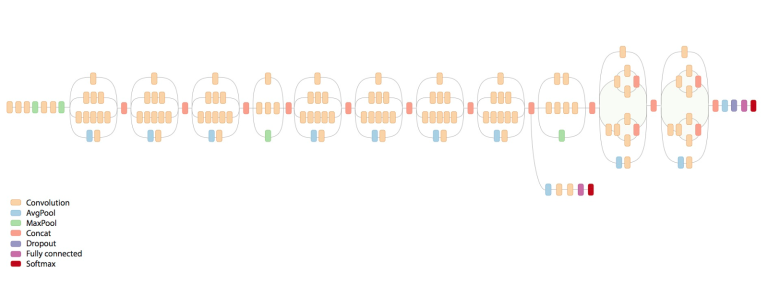
\includegraphics[width=0.8\textwidth]{inceptionv3.png} % adjust width
	\caption{\textit{Inception v3 architecture}} % optional
	\label{fig:inceptionv3}
\end{figure}

\section{The dataset}
\label{sec:dataset}
Both training and test images are taken from the Sapienza MarDCT dataset, a wide database of images and videos containing data coming from multiple video sources (fixed, zooming, and Pan-Tilt-Zoom cameras) and from different scenarios: in particular I have used the images of 24 different categories of boats navigating in the italian city of Venice and extracted by the ARGOS system. This dataset is already divided into training and test images: however, some preprocessing was needed in order to handle the different structure of the two sets of images and also because there were some multi-labeled images in the test set: in particular, the training set was organized in 24 folders, each containing a specific class of images; the name of each folder is the name of the class, i.e. the boat type; the class "water" actually contains a set of false positives images. The test set is provided, instead, as a unique (no folders!) collection of images; thanks to the file \textit{ground\_truth.txt}, however, it is possible to associate each file to a specific label. As already said, some images contain fragments of boats (these images are labeled as \textit{partial}) or two or more boats of different types (multiple label). I have decided to simply skip these test images.

\subsection{Preprocessing}
\label{sec:preprocessing}

% summary of the preprocessing phase preprocessing.py
First of all I have decided to limit the number of classes to 18 (out of the total 24), excluding all classes with less than 10 images. Figure \ref{fig:labels} lists all the classes that I have included in the training phase. At the end of the preprocessing phase the number the dataset was:
\begin{itemize}
	\item \textbf{3810}\footnote{cfr. figure \ref{fig:labels} to see the number of images per label} training images
	\item \textbf{1252}\footnote{the number of test images is actually is 1969, but as stated in section \ref{sec:dataset} I have filtered the images with partial or multiple labels and the false positives (i.e. \textit{water} label)} test images
\end{itemize}

\subsubsection{Extract features}
\begin{figure}[!ht]
	\centering % optional
	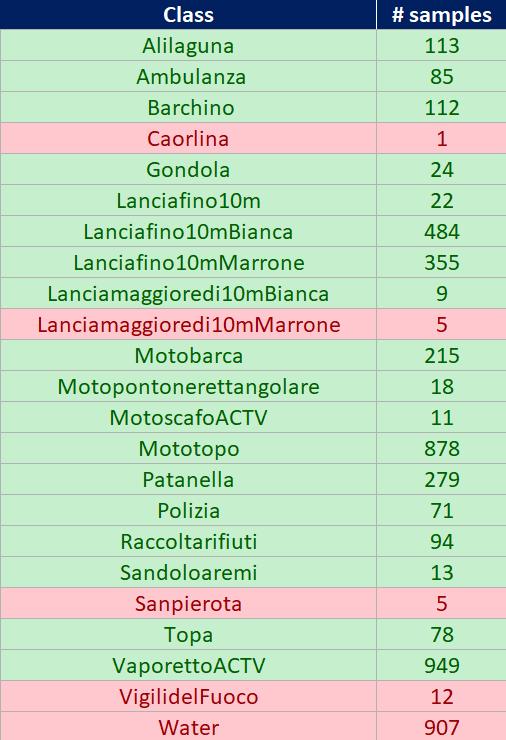
\includegraphics[width=0.5\textwidth]{labels.png} % adjust width
	\caption{\textit{Boat classes from dataset MarDCT}} % optional
	\label{fig:labels}
\end{figure}
Once the pretrained graph was taken into main memory from disk, the images have been fed to a TensorFlow implementation of Inception v3, downloaded from the official repository, with the classification layer removed in order to produce a set of labeled feature vectors of 2048 floats: this \textit{next-to-last} layer is a tensor called 'pool\_3:0'. Inception is, indeed, a complex model (see figure \ref{fig:inceptionv3}) made up by a lot of submodules: namely the Inception modules. Each module implements a set of primitives (e.g. filtering, max pooling, etc.), so what I have done is simply remove the last layer of the network and collect the feature vectors.

\section{Classification}
% summary of classifier.py
\subsubsection{t-sne features}
I have carried out dimensionality reduction on the 2048-D feature vector using t-distributed stochastic neighbor embedding (\textbf{t-SNE}) to transform the input features into a 2-D feature which is easy to visualize. The t-SNE is used as an informative step: if the same color (i.e. label) points are mostly clustered together there is a high chance that we could use the features to train a classifier with high accuracy. Figure \ref{fig:tsne} shows the result of this phase.

\begin{figure}[!ht]
	\centering % optional
	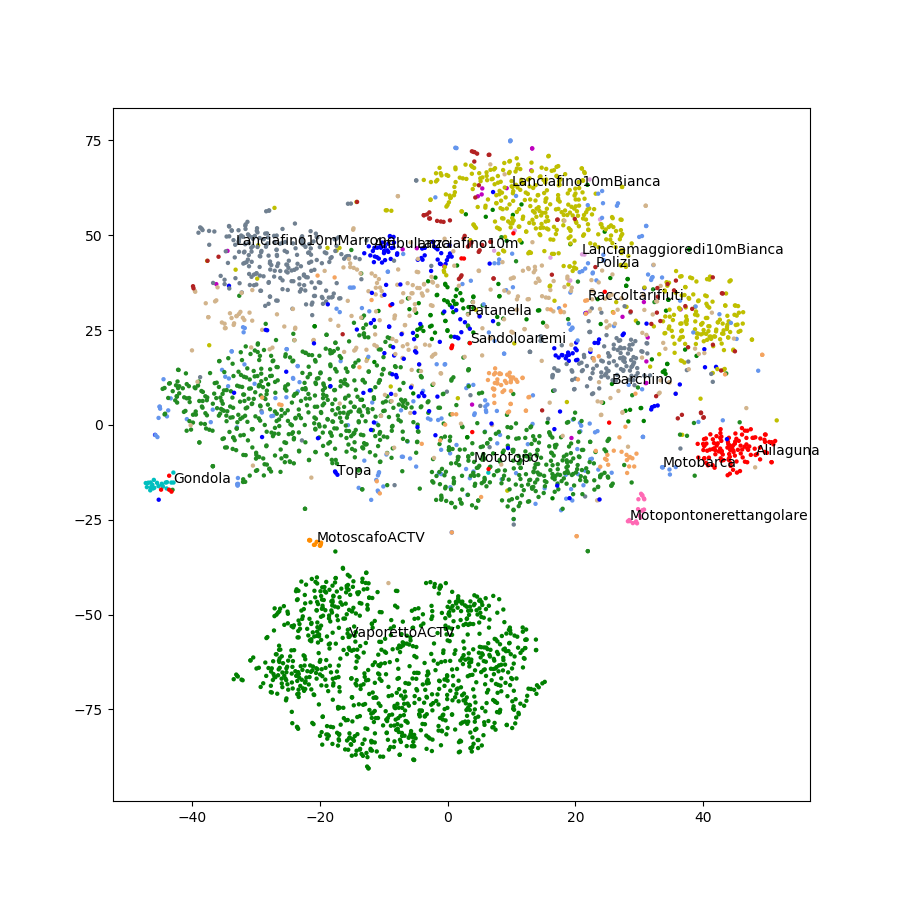
\includegraphics[width=1\textwidth]{../code/output/features.png} % adjust width
	\caption{\textit{t-SNE features extracted from Inception v3.}} % optional
	\label{fig:tsne}
\end{figure}

\subsection{Running the classifiers}
For each model (for the complete list see \ref{sec:models}) I have run the proper classifier. In most cases I have simply used the default configuration, however for a complete list of parameters passed to each classifier see the file \textit{main.py}.

\section{The results}
\label{sec:results}
I have computed the accuracy and the precision for each classifier, and I have finally plotted the confusion (and not normalized) matrices. They are shown in the following images. All the following results have been computed with the cross validation process. The accuracy and the precision have been computed as the average of the above metrics obtained after each phase of evaluation. Also the confusion matrices have been built during the cross validation process: it was computed weighted average of the confusion matrices for each fold. Remembering that:
$
\newline\newline
\mbox{Accuracy}:= \frac{|\mbox{true positives}| + |\mbox{true negatives}|}{|\mbox{instances}|}
\newline\newline
\mbox{Precision}:= \frac{|\mbox{true positives}|}{|\mbox{predicted positives}|}
\newline\newline
$
I am going to show the results obtained for all the models: they are also plotted in figure \ref{fig:metrics}.
\subsection{Metrics}
\begin{figure}[!ht]
	\centering % optional
	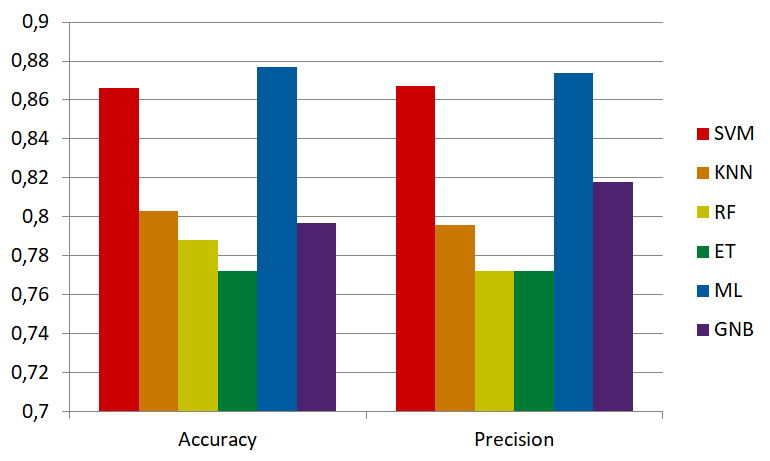
\includegraphics[width=0.8\textwidth]{metrics.png} % adjust width
	\caption{\textit{Precision and accuracy of the classifiers}} % optional
	\label{fig:metrics}
\end{figure}
\subsubsection{SVM}
The accuracy was 86.6\% and the precision was 86.7\%
\subsubsection{KNN}
The accuracy was 80.3\% and the precision was 79.6\%

\begin{figure}[!ht]
	\centering
	\begin{minipage}{.5\textwidth}
		\centering
		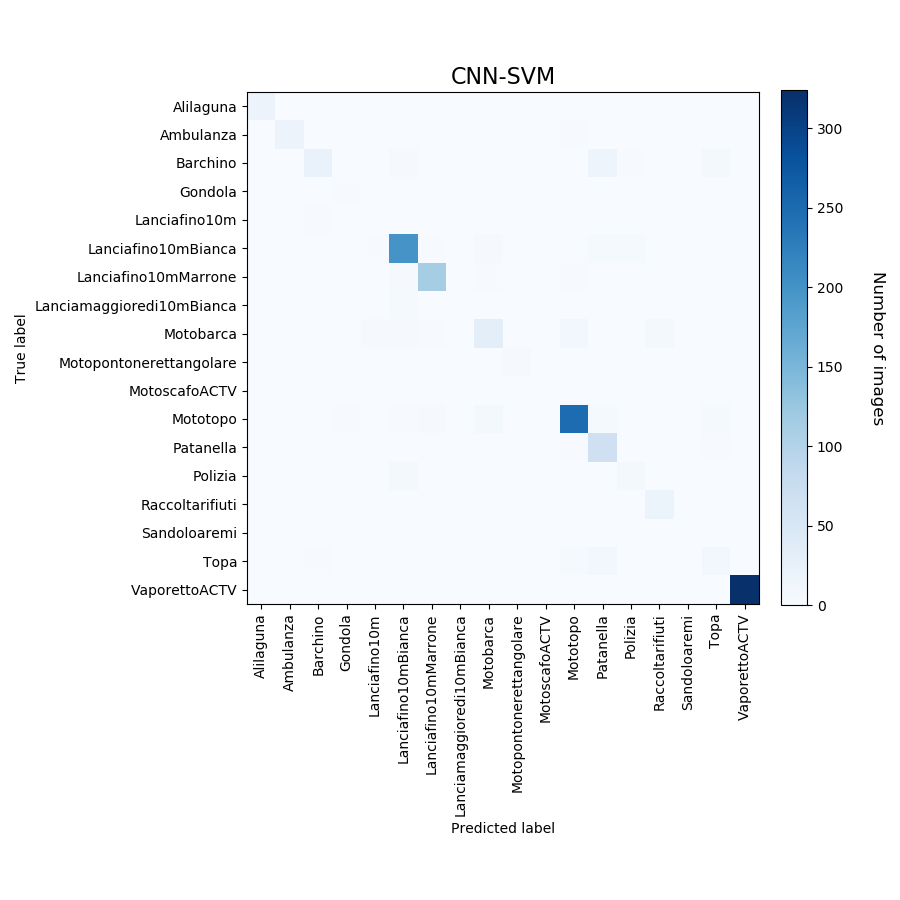
\includegraphics[width=.8\linewidth]{../code/output/CNN-SVM.png}
		\caption{SVM confusion matrix} % optional
		\label{fig:cnf_svm}
	\end{minipage}%
	\begin{minipage}{.5\textwidth}
		\centering
		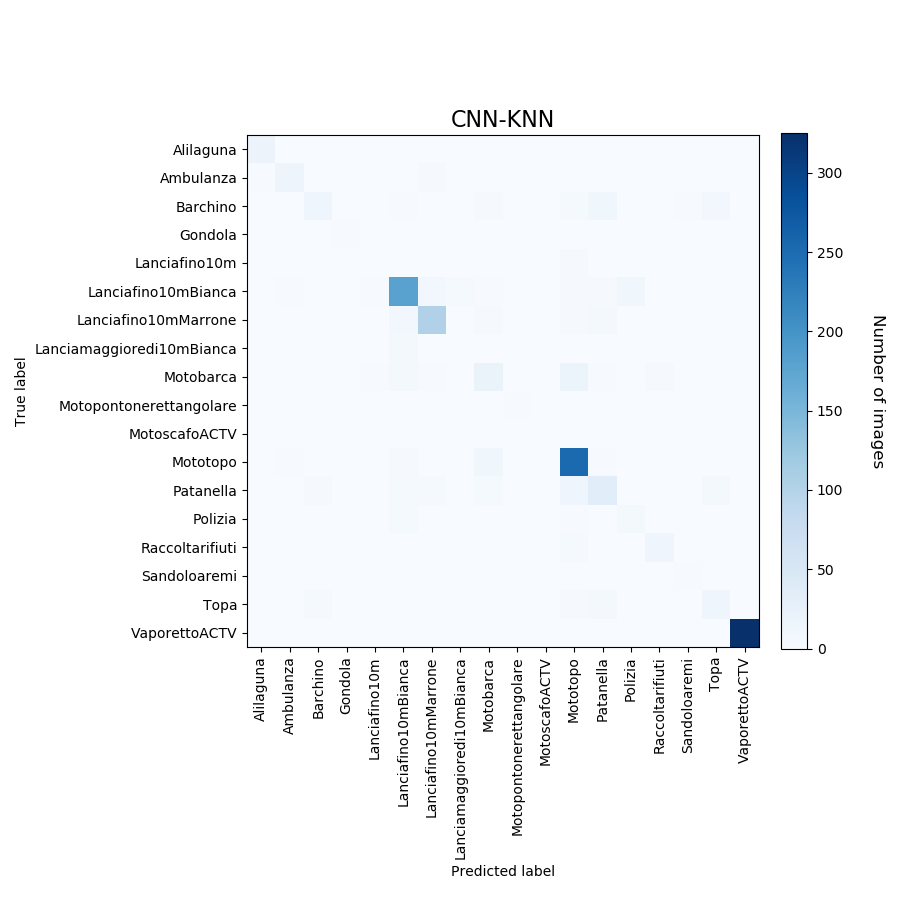
\includegraphics[width=.8\linewidth]{../code/output/CNN-KNN.png}
		\caption{KNN confusion matrix} % optional
		\label{fig:cnf_knn}
	\end{minipage}
\end{figure}

\subsubsection{RF}
The accuracy was 78.8\% and the precision was 77.2\%
\subsubsection{ET}
The accuracy was 77.2\% and the precision was 77.2\%

\begin{figure}[!ht]
	\centering
	\begin{minipage}{.5\textwidth}
		\centering
		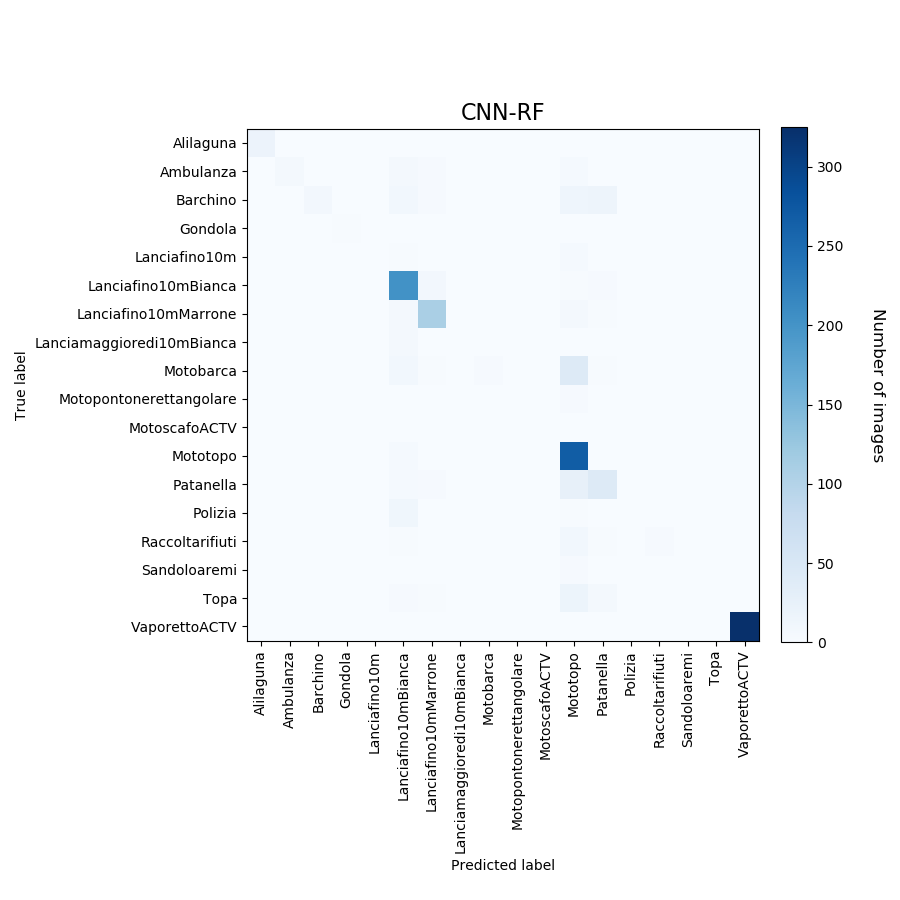
\includegraphics[width=.8\linewidth]{../code/output/CNN-RF.png}
		\caption{RF confusion matrix} % optional
		\label{fig:cnf_rf}
	\end{minipage}%
	\begin{minipage}{.5\textwidth}
		\centering
		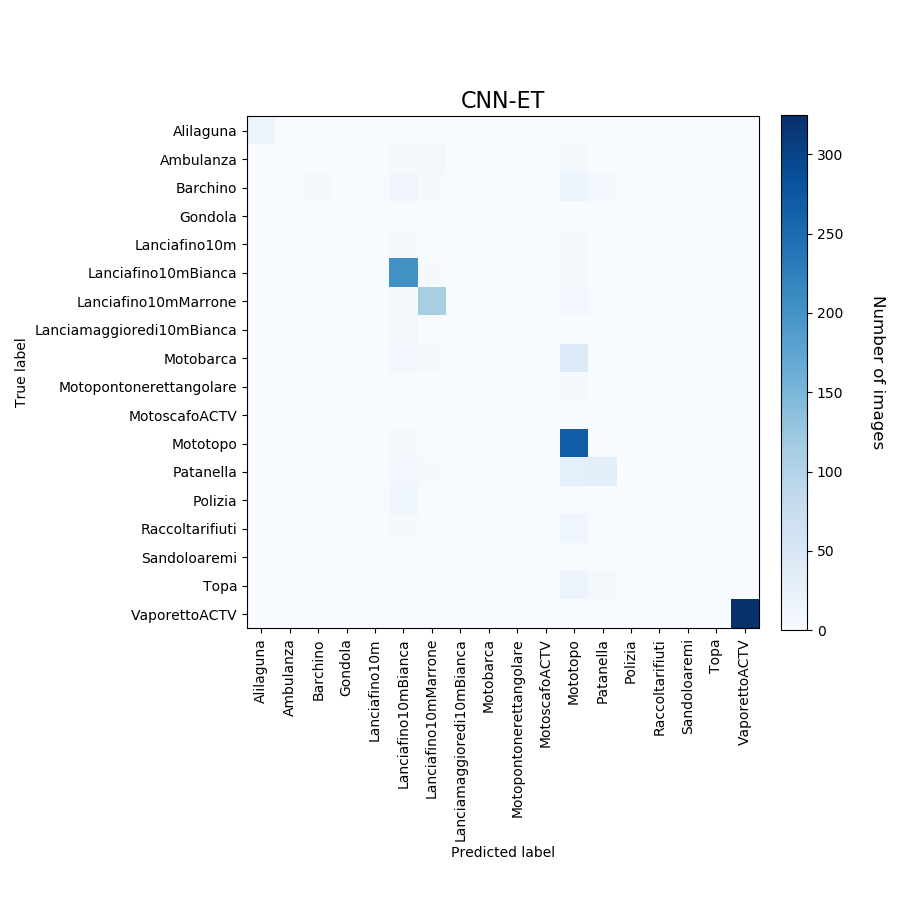
\includegraphics[width=.8\linewidth]{../code/output/CNN-ET.png}
		\caption{ET confusion matrix} % optional
		\label{fig:cnf_et}
	\end{minipage}
\end{figure}

\subsubsection{ML}
The accuracy was 87.7\% and the precision was 87.4\%
\subsubsection{GNB}
The accuracy was 79.7\% and the precision was 81.8\%

\begin{figure}[!ht]
	\centering
	\begin{minipage}{.5\textwidth}
		\centering
		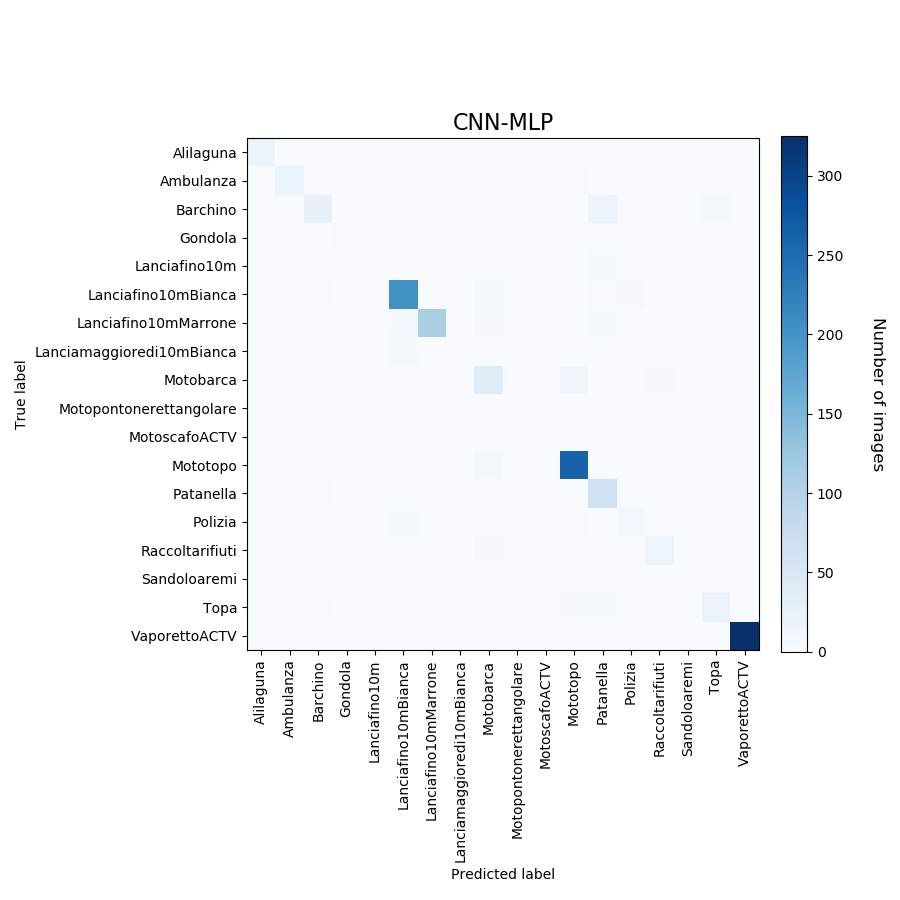
\includegraphics[width=.8\linewidth]{../code/output/CNN-MLP.png}
		\caption{ML confusion matrix} % optional
		\label{fig:cnf_mlp}
	\end{minipage}%
	\begin{minipage}{.5\textwidth}
		\centering
		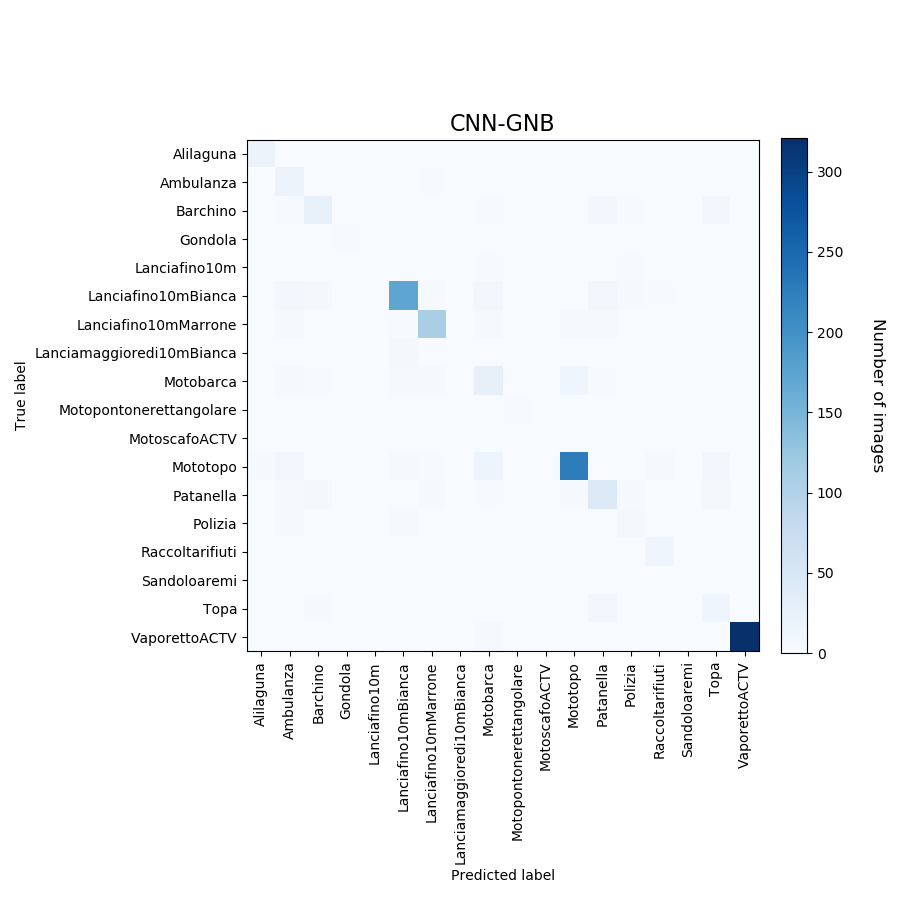
\includegraphics[width=.8\linewidth]{../code/output/CNN-GNB.png}
		\caption{GNB confusion matrix} % optional
		\label{fig:cnf_gnb}
	\end{minipage}
\end{figure}

\section{Conclusions}
Figure \ref{fig:metrics} shows that Multi-Layer Perceptron (MLP) and Support Vector Machine (SVM) classifiers reach very good results in both accuracy and precision, with values higher than 0.86. The other classifiers, instead, reach levels of accuracy and precision under the 0.8 threshold.

\newpage
\begin{thebibliography}{10}
	
	% bibitem for book
	\bibitem{Main Book}
	Tom M. Mitchell \textsl{Machine Learning}.
	
	\bibitem{Inception}
	C. Szegedy, V. Vanhoucke, S. Ioffe, J. Shlens, Z. Wojna
	\textsl{Rethinking the Inception Architecture for Computer Vision}
	
\end{thebibliography}
\end{document}